\subsection{LA48 Four-Level Paging}

When (:ref:base.control_registers.PTCR.LA57:) is zero, bits \texttt{63..48} of the (:term:base.terms.linear_address:) must equal the sign extension of bit
\texttt{47}. Bits \texttt{47..39}, \texttt{38..30}, \texttt{29..21}, and \texttt{20..12} select the L4, L3, L2,
and L1 entries respectively. A byte-addressed leaf may terminate the walk at any of those levels; all bits below
the terminating level\textquotesingle{}s index form its offset. The L4 table is the root table named by (:ref:base.control_registers.PTCR.ROOT_PAGE:).

\begin{center}\vspace{3pt}
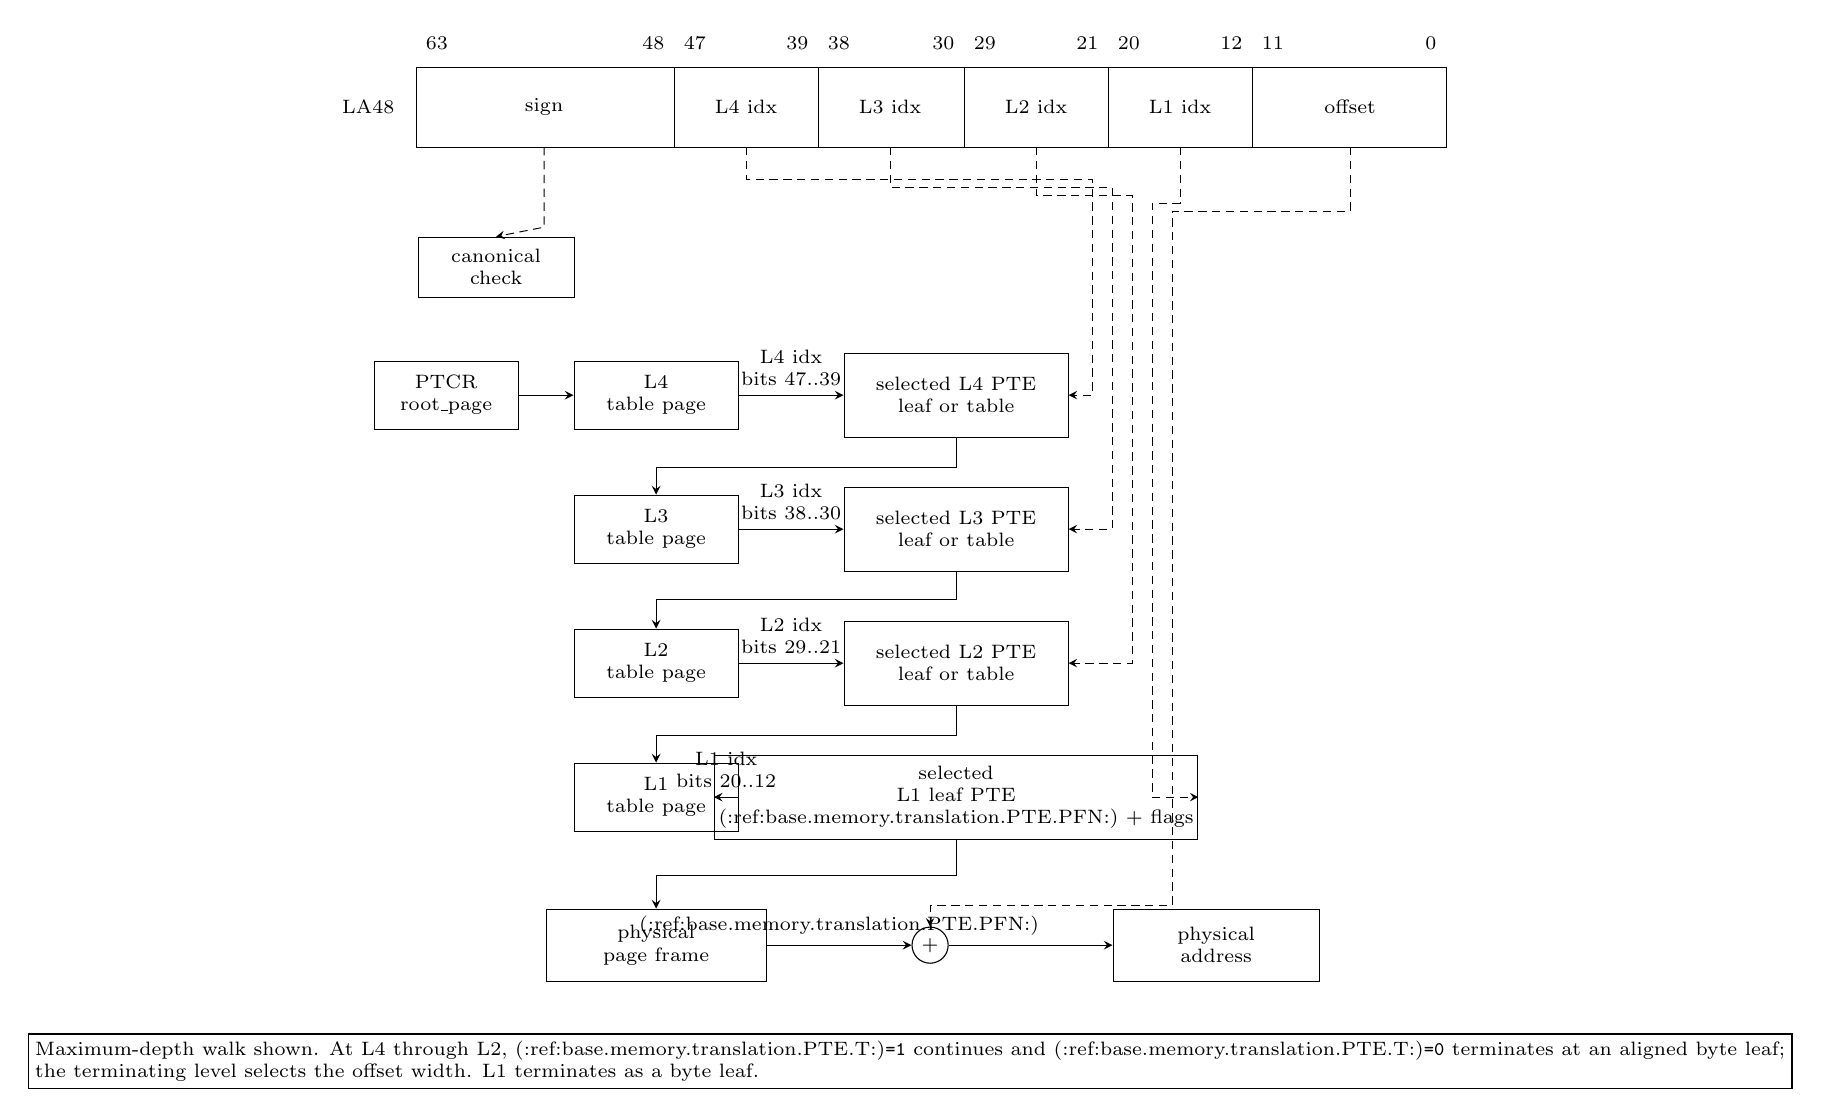
\begin{tikzpicture}[x=1in,y=1in,every node/.style={font=\scriptsize},>=stealth]
\node[anchor=east] at (0.49,6.22) {LA48};
\node[anchor=south west] at (0.55,6.46) {63};
\node[anchor=south east] at (1.84,6.46) {48};
\draw (0.55,6.02) rectangle (1.84,6.42);
\node[align=center] at (1.19,6.22) {sign};
\node[anchor=south west] at (1.84,6.46) {47};
\node[anchor=south east] at (2.56,6.46) {39};
\draw (1.84,6.02) rectangle (2.56,6.42);
\node[align=center] at (2.20,6.22) {L4 idx};
\node[anchor=south west] at (2.56,6.46) {38};
\node[anchor=south east] at (3.29,6.46) {30};
\draw (2.56,6.02) rectangle (3.29,6.42);
\node[align=center] at (2.92,6.22) {L3 idx};
\node[anchor=south west] at (3.29,6.46) {29};
\node[anchor=south east] at (4.01,6.46) {21};
\draw (3.29,6.02) rectangle (4.01,6.42);
\node[align=center] at (3.65,6.22) {L2 idx};
\node[anchor=south west] at (4.01,6.46) {20};
\node[anchor=south east] at (4.73,6.46) {12};
\draw (4.01,6.02) rectangle (4.73,6.42);
\node[align=center] at (4.37,6.22) {L1 idx};
\node[anchor=south west] at (4.73,6.46) {11};
\node[anchor=south east] at (5.70,6.46) {0};
\draw (4.73,6.02) rectangle (5.70,6.42);
\node[align=center] at (5.22,6.22) {offset};
\node[draw,align=center,minimum width=0.78in,minimum height=0.30in] (canon) at (0.95,5.42) {canonical\\check};
\draw[->,black,densely dashed,line width=0.35pt] (1.19,6.02) -- (1.19,5.62) -- (canon.north);
\node[draw,align=center,minimum width=0.82in,minimum height=0.34in,inner sep=1.5pt] (tbl0) at (1.75,4.78) {L4\\table page};
\node[draw,align=center,minimum width=1.12in,minimum height=0.42in,inner sep=1.5pt] (ent0) at (3.25,4.78) {selected L4 PTE\\leaf or table};
\node[draw,align=center,minimum width=0.72in,minimum height=0.34in,inner sep=1.5pt] (root) at (0.70,4.78) {PTCR\\root\_page};
\draw[->] (root.east) -- (tbl0.west);
\draw[->] (tbl0.east) -- node[above,align=center,font=\scriptsize] {L4 idx\\bits 47..39} (ent0.west);
\draw[->,black,densely dashed,line width=0.35pt] (2.20,6.02) -- (2.20,5.86) -- (3.93,5.86) -- (3.93,4.78) -- (ent0.east);
\node[draw,align=center,minimum width=0.82in,minimum height=0.34in,inner sep=1.5pt] (tbl1) at (1.75,4.11) {L3\\table page};
\node[draw,align=center,minimum width=1.12in,minimum height=0.42in,inner sep=1.5pt] (ent1) at (3.25,4.11) {selected L3 PTE\\leaf or table};
\draw[->] (ent0.south) -- (3.25,4.42) -- (1.75,4.42) -- (tbl1.north);
\draw[->] (tbl1.east) -- node[above,align=center,font=\scriptsize] {L3 idx\\bits 38..30} (ent1.west);
\draw[->,black,densely dashed,line width=0.35pt] (2.92,6.02) -- (2.92,5.82) -- (4.03,5.82) -- (4.03,4.11) -- (ent1.east);
\node[draw,align=center,minimum width=0.82in,minimum height=0.34in,inner sep=1.5pt] (tbl2) at (1.75,3.44) {L2\\table page};
\node[draw,align=center,minimum width=1.12in,minimum height=0.42in,inner sep=1.5pt] (ent2) at (3.25,3.44) {selected L2 PTE\\leaf or table};
\draw[->] (ent1.south) -- (3.25,3.76) -- (1.75,3.76) -- (tbl2.north);
\draw[->] (tbl2.east) -- node[above,align=center,font=\scriptsize] {L2 idx\\bits 29..21} (ent2.west);
\draw[->,black,densely dashed,line width=0.35pt] (3.65,6.02) -- (3.65,5.78) -- (4.13,5.78) -- (4.13,3.44) -- (ent2.east);
\node[draw,align=center,minimum width=0.82in,minimum height=0.34in,inner sep=1.5pt] (tbl3) at (1.75,2.77) {L1\\table page};
\node[draw,align=center,minimum width=1.12in,minimum height=0.42in,inner sep=1.5pt] (ent3) at (3.25,2.77) {selected\\L1 leaf PTE\\(:ref:base.memory.translation.PTE.PFN:) + flags};
\draw[->] (ent2.south) -- (3.25,3.08) -- (1.75,3.08) -- (tbl3.north);
\draw[->] (tbl3.east) -- node[above,align=center,font=\scriptsize] {L1 idx\\bits 20..12} (ent3.west);
\draw[->,black,densely dashed,line width=0.35pt] (4.37,6.02) -- (4.37,5.74) -- (4.23,5.74) -- (4.23,2.77) -- (ent3.east);
\node[draw,align=center,minimum width=1.10in,minimum height=0.36in] (frame) at (1.75,2.03) {physical\\page frame};
\draw[->] (ent3.south) -- (3.25,2.38) -- (1.75,2.38) -- (frame.north);
\node[draw,circle,inner sep=1.8pt] (plus) at (3.12,2.03) {+};
\node[draw,align=center,minimum width=1.03in,minimum height=0.36in] (phys) at (4.55,2.03) {physical\\address};
\draw[->] (frame.east) -- node[above] {(:ref:base.memory.translation.PTE.PFN:)} (plus.west);
\draw[->] (plus.east) -- (phys.west);
\draw[->,black,densely dashed,line width=0.35pt] (5.22,6.02) -- (5.22,5.70) -- (4.33,5.70) -- (4.33,2.23) -- (3.12,2.23) -- (plus.north);
\node[draw,align=left,minimum width=4.55in,inner sep=2.5pt] at (3.02,1.45) {Maximum-depth walk shown. At L4 through L2, (:ref:base.memory.translation.PTE.T:)\texttt{=1} continues and (:ref:base.memory.translation.PTE.T:)\texttt{=0} terminates at an aligned byte leaf;\\the terminating level selects the offset width. L1 terminates as a byte leaf.};
\end{tikzpicture}
\BedrockFigureCaption{LA48 Four-Level Page Walk}
\end{center}


\clearpage
